%%%%%%%% ICML 2021 EXAMPLE LATEX SUBMISSION FILE %%%%%%%%%%%%%%%%%

\documentclass{article}

% Recommended, but optional, packages for figures and better typesetting:
\usepackage{microtype}
\usepackage{graphicx}
\usepackage{subfigure}
\usepackage{booktabs} % for professional tables

% hyperref makes hyperlinks in the resulting PDF.
% If your build breaks (sometimes temporarily if a hyperlink spans a page)
% please comment out the following usepackage line and replace
% \usepackage{icml2021} with \usepackage[nohyperref]{icml2021} above.
\usepackage{hyperref}

% Attempt to make hyperref and algorithmic work together better:
\newcommand{\theHalgorithm}{\arabic{algorithm}}

% Use the following line for the initial blind version submitted for review:
% \usepackage{icml2021}

% If accepted, instead use the following line for the camera-ready submission:
\usepackage[accepted]{icml2021}

% The \icmltitle you define below is probably too long as a header.
% Therefore, a short form for the running title is supplied here:
\icmltitlerunning{Image Animation with Keypoint Mask}

\begin{document}

\twocolumn[
\icmltitle{Image Animation with Keypoint Mask}
% It is OKAY to include author information, even for blind
% submissions: the style file will automatically remove it for you
% unless you've provided the [accepted] option to the icml2021
% package.

% List of affiliations: The first argument should be a (short)
% identifier you will use later to specify author affiliations
% Academic affiliations should list Department, University, City, Region, Country
% Industry affiliations should list Company, City, Region, Country

% You can specify symbols, otherwise they are numbered in order.
% Ideally, you should not use this facility. Affiliations will be numbered
% in order of appearance and this is the preferred way.
\icmlsetsymbol{equal}{*}

\begin{icmlauthorlist}
\icmlauthor{Or Toledano}{tlv}
\end{icmlauthorlist}

\icmlaffiliation{tlv}{Tel Aviv University}

\icmlcorrespondingauthor{Or Toledano}{ortoledano@protonmail.com}

% You may provide any keywords that you
% find helpful for describing your paper; these are used to populate
% the "keywords" metadata in the PDF but will not be shown in the document
\icmlkeywords{Machine Learning, ICML}

\vskip 0.3in
]

% this must go after the closing bracket ] following \twocolumn[ ...
% This command actually creates the footnote in the first column
% listing the affiliations and the copyright notice.
% The command takes one argument, which is text to display at the start of the footnote.
% The \icmlEqualContribution command is standard text for equal contribution.
% Remove it (just {}) if you do not need this facility.
\printAffiliationsAndNotice{}  % leave blank if no need to mention equal contribution
%\printAffiliationsAndNotice{\icmlEqualContribution} % otherwise use the standard text.

\begin{abstract}
TODO OR
important
transgaga structure
realtime
\cite{siarohin2020order}
\end{abstract}

\section{Electronic Submission}
\label{submission}
\textbf{Paper Deadline:} The deadline for paper submission that is
advertised on the conference website is strict. If your full,
anonymized, submission does not reach us on time, it will not be
considered for publication.

\textbf{Anonymous Submission:} ICML uses double-blind review: no identifying
author information may appear on the title page or in the paper

\textbf{Simultaneous Submission:} ICML will not accept any paper which,
at the time of submission, is under review for another conference or
has already been published. This policy also applies to papers that
overlap substantially in technical content with conference papers
under review or previously published. ICML submissions must not be
submitted to other conferences and journals during ICML's review
period.
%Authors may submit to ICML substantially different versions of journal papers
%that are currently under review by the journal, but not yet accepted
%at the time of submission.
Informal publications, such as technical
reports or papers in workshop proceedings which do not appear in
print, do not fall under these restrictions.

\medskip


It is a zero following the ``-G'', which tells dvips to use
the config.pdf file. Newer \TeX\ distributions don't always need this
option.

Using \texttt{pdflatex} rather than \texttt{latex}, often gives better
results. This program avoids the Type-3 font problem, and supports more
advanced features in the \texttt{microtype} package.

\textbf{Graphics files} should be a reasonable size, and included from
an appropriate format. Use vector formats (.eps/.pdf) for plots,
lossless bitmap formats (.png) for raster graphics with sharp lines, and
jpeg for photo-like images.

The style file uses the \texttt{hyperref} package to make clickable
links in documents. If this causes problems for you, add
\texttt{nohyperref} as one of the options to the \texttt{icml2021}
usepackage statement.

\subsubsection{Camera-Ready Author Information}
\label{final author}

If a paper is accepted, a final camera-ready copy must be prepared.
\subsection{Abstract}

The paper abstract should begin in the left column,

\subsubsection{Paragraphs and Footnotes}

Within each section or subsection, you should further partition the
paper into paragraphs. Do not indent the first line of a given
paragraph, but insert a blank line between succeeding ones.

You can use footnotes\footnote{Footnotes
should be complete sentences.} to provide readers with additional
information about a topic without interrupting the flow of the paper.
Indicate footnotes with a number in the text where the point is most
relevant. Place the footnote in 9~point type at the bottom of the
column in which it appears. Precede the first footnote in a column
with a horizontal rule of 0.8~inches.\footnote{Multiple footnotes can
appear in each column, in the same order as they appear in the text,
but spread them across columns and pages if possible.}

\begin{figure}[ht]
\vskip 0.2in
\begin{center}
\centerline{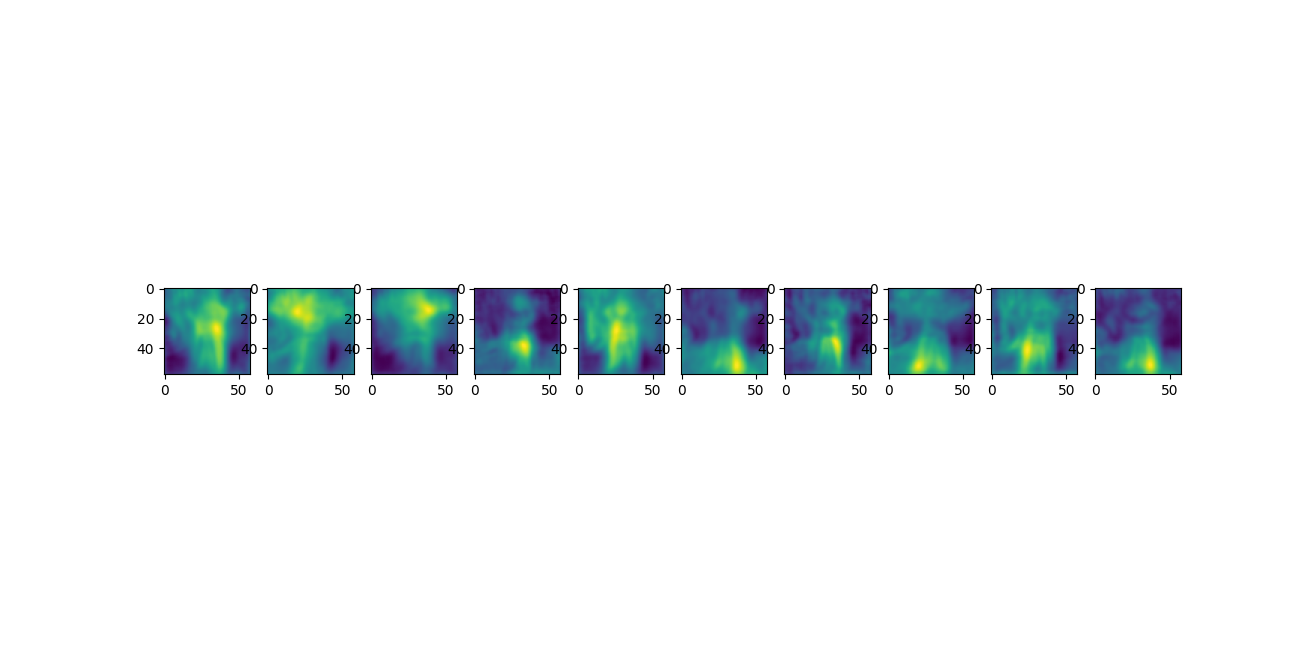
\includegraphics[width=\columnwidth]{mask_10kp}}
\caption{
$K$ channels of the keypoint detector network used in
\cite{siarohin2020order}, before the softmax activation. Our main motion
prior in this project.
}
\label{mask-10kp}
\end{center}
\vskip -0.2in
\end{figure}

\subsection{Figures}

emph{after} the graphics, with at least 0.1~inches of space before
the caption and 0.1~inches after it, as in
9~point type and centered unless it runs two or more lines, in which
case it should be flush left. You may float figures to the top or
bottom of a column, and you may set wide figures across both columns
(use the environment \texttt{figure*} in \LaTeX). Always place
two-column figures at the top or bottom of the page.

\subsection{Algorithms}

If you are using \LaTeX, please use the ``algorithm'' and ``algorithmic''
environments to format pseudocode. These require
the corresponding stylefiles, algorithm.sty and
algorithmic.sty, which are supplied with this package.


\subsection{Tables}

You may also want to include tables that summarize material. Like
figures, these should be centered, legible, and numbered consecutively.
However, place the title \emph{above} the table with at least
0.1~inches of space before the title and the same after it, as in
Table~\ref{sample-table}. The table title should be set in 9~point
type and centered unless it runs two or more lines, in which case it
should be flush left.

% Note use of \abovespace and \belowspace to get reasonable spacing
% above and below tabular lines.

\begin{table}[t]
\caption{Accuracy TODO Dov}
\label{sample-table}
\vskip 0.15in
\begin{center}
\begin{small}
\begin{sc}
\begin{tabular}{lcccr}
\toprule
Data set & Naive & Flexible & Better? \\
\midrule
Breast    & 95.9$\pm$ 0.2& 96.7$\pm$ 0.2& $\surd$ \\
Cleveland & 83.3$\pm$ 0.6& 80.0$\pm$ 0.6& $\times$\\
Glass2    & 61.9$\pm$ 1.4& 83.8$\pm$ 0.7& $\surd$ \\
Credit    & 74.8$\pm$ 0.5& 78.3$\pm$ 0.6&         \\
Horse     & 73.3$\pm$ 0.9& 69.7$\pm$ 1.0& $\times$\\
Meta      & 67.1$\pm$ 0.6& 76.5$\pm$ 0.5& $\surd$ \\
Pima      & 75.1$\pm$ 0.6& 73.9$\pm$ 0.5&         \\
Vehicle   & 44.9$\pm$ 0.6& 61.5$\pm$ 0.4& $\surd$ \\
\bottomrule
\end{tabular}
\end{sc}
\end{small}
\end{center}
\vskip -0.1in
\end{table}

Tables contain textual material, whereas figures contain graphical material.
Specify the contents of each row and column in the table's topmost
row. Again, you may float tables to a column's top or bottom, and set
wide tables across both columns. Place two-column tables at the
top or bottom of the page.

\section*{Software and Data}

If a paper is accepted, we strongly encourage the publication of software and data with the
camera-ready version of the paper whenever appropriate. This can be
done by including a URL in the camera-ready copy. However, \textbf{do not}
include URLs that reveal your institution or identity in your
submission for review. Instead, provide an anonymous URL or upload
the material as ``Supplementary Material'' into the CMT reviewing
system. Note that reviewers are not required to look at this material
when writing their review.

% In the unusual situation where you want a paper to appear in the
% references without citing it in the main text, use \nocite
% \nocite{langley00}

\bibliography{animation-with-keypoint-mask}
\bibliographystyle{icml2021}

\end{document}
